\section{Nanoribbon}
\label{sec:nanoribbon}

In this section, we apply our code to the case of honeycomb lattice with boundary conditions corresponding to a nanoribbon.

A nanoribbon is much longer on one direction than on the other, i.e. $l \gg w$. 
This condition corresponds to taking $N_x \gg N_y$ in our conventions (see figure (\ref{fig:nanoribbon}), where this condition is, of course, not obeyed solely for the sake of giving a visual representation of the boundary conditions, and the numbering system).

We use three coordinates to label each site on the honeycomb lattice, by taking advantage of its bipartite nature.
Regarding the honeycomb lattice as two interpenetrating triangular sublattices $A$ and $B$, we take the axes $x$ and $y$ to be along the primitive vectors of each triangular sublattice.
Along the $x$-direction, the ribbon is supposed to be very long, which justifies the fact that we take \acp{PBC}.
In contrast, in the narrow $y$-direction we take \acp{OBC}.
To number the sites on the ribbon, we introduce an additional coordinate labeling the sublattice: $z = 0$, if the site is in sublattice $A$, and $z = 1$ if the site is in sublattice $B$.
We then adopt the numbering convention for the sites $i = 1, ..., 2 N_x N_y$ of the lattice $\mathcal{L}$:

\begin{equation}\label{eq:numbering}
i (x, y, z) = N_x N_y z + N_x y + x,
\end{equation}
where $x = 0, ..., N_x - 1$, $y = 0, ..., N_y - 1$, and $z = 0, 1$ define each element $\bm r = (x, y, z) \in \mathcal{L}$.

\begin{figure}[H]
	\centering
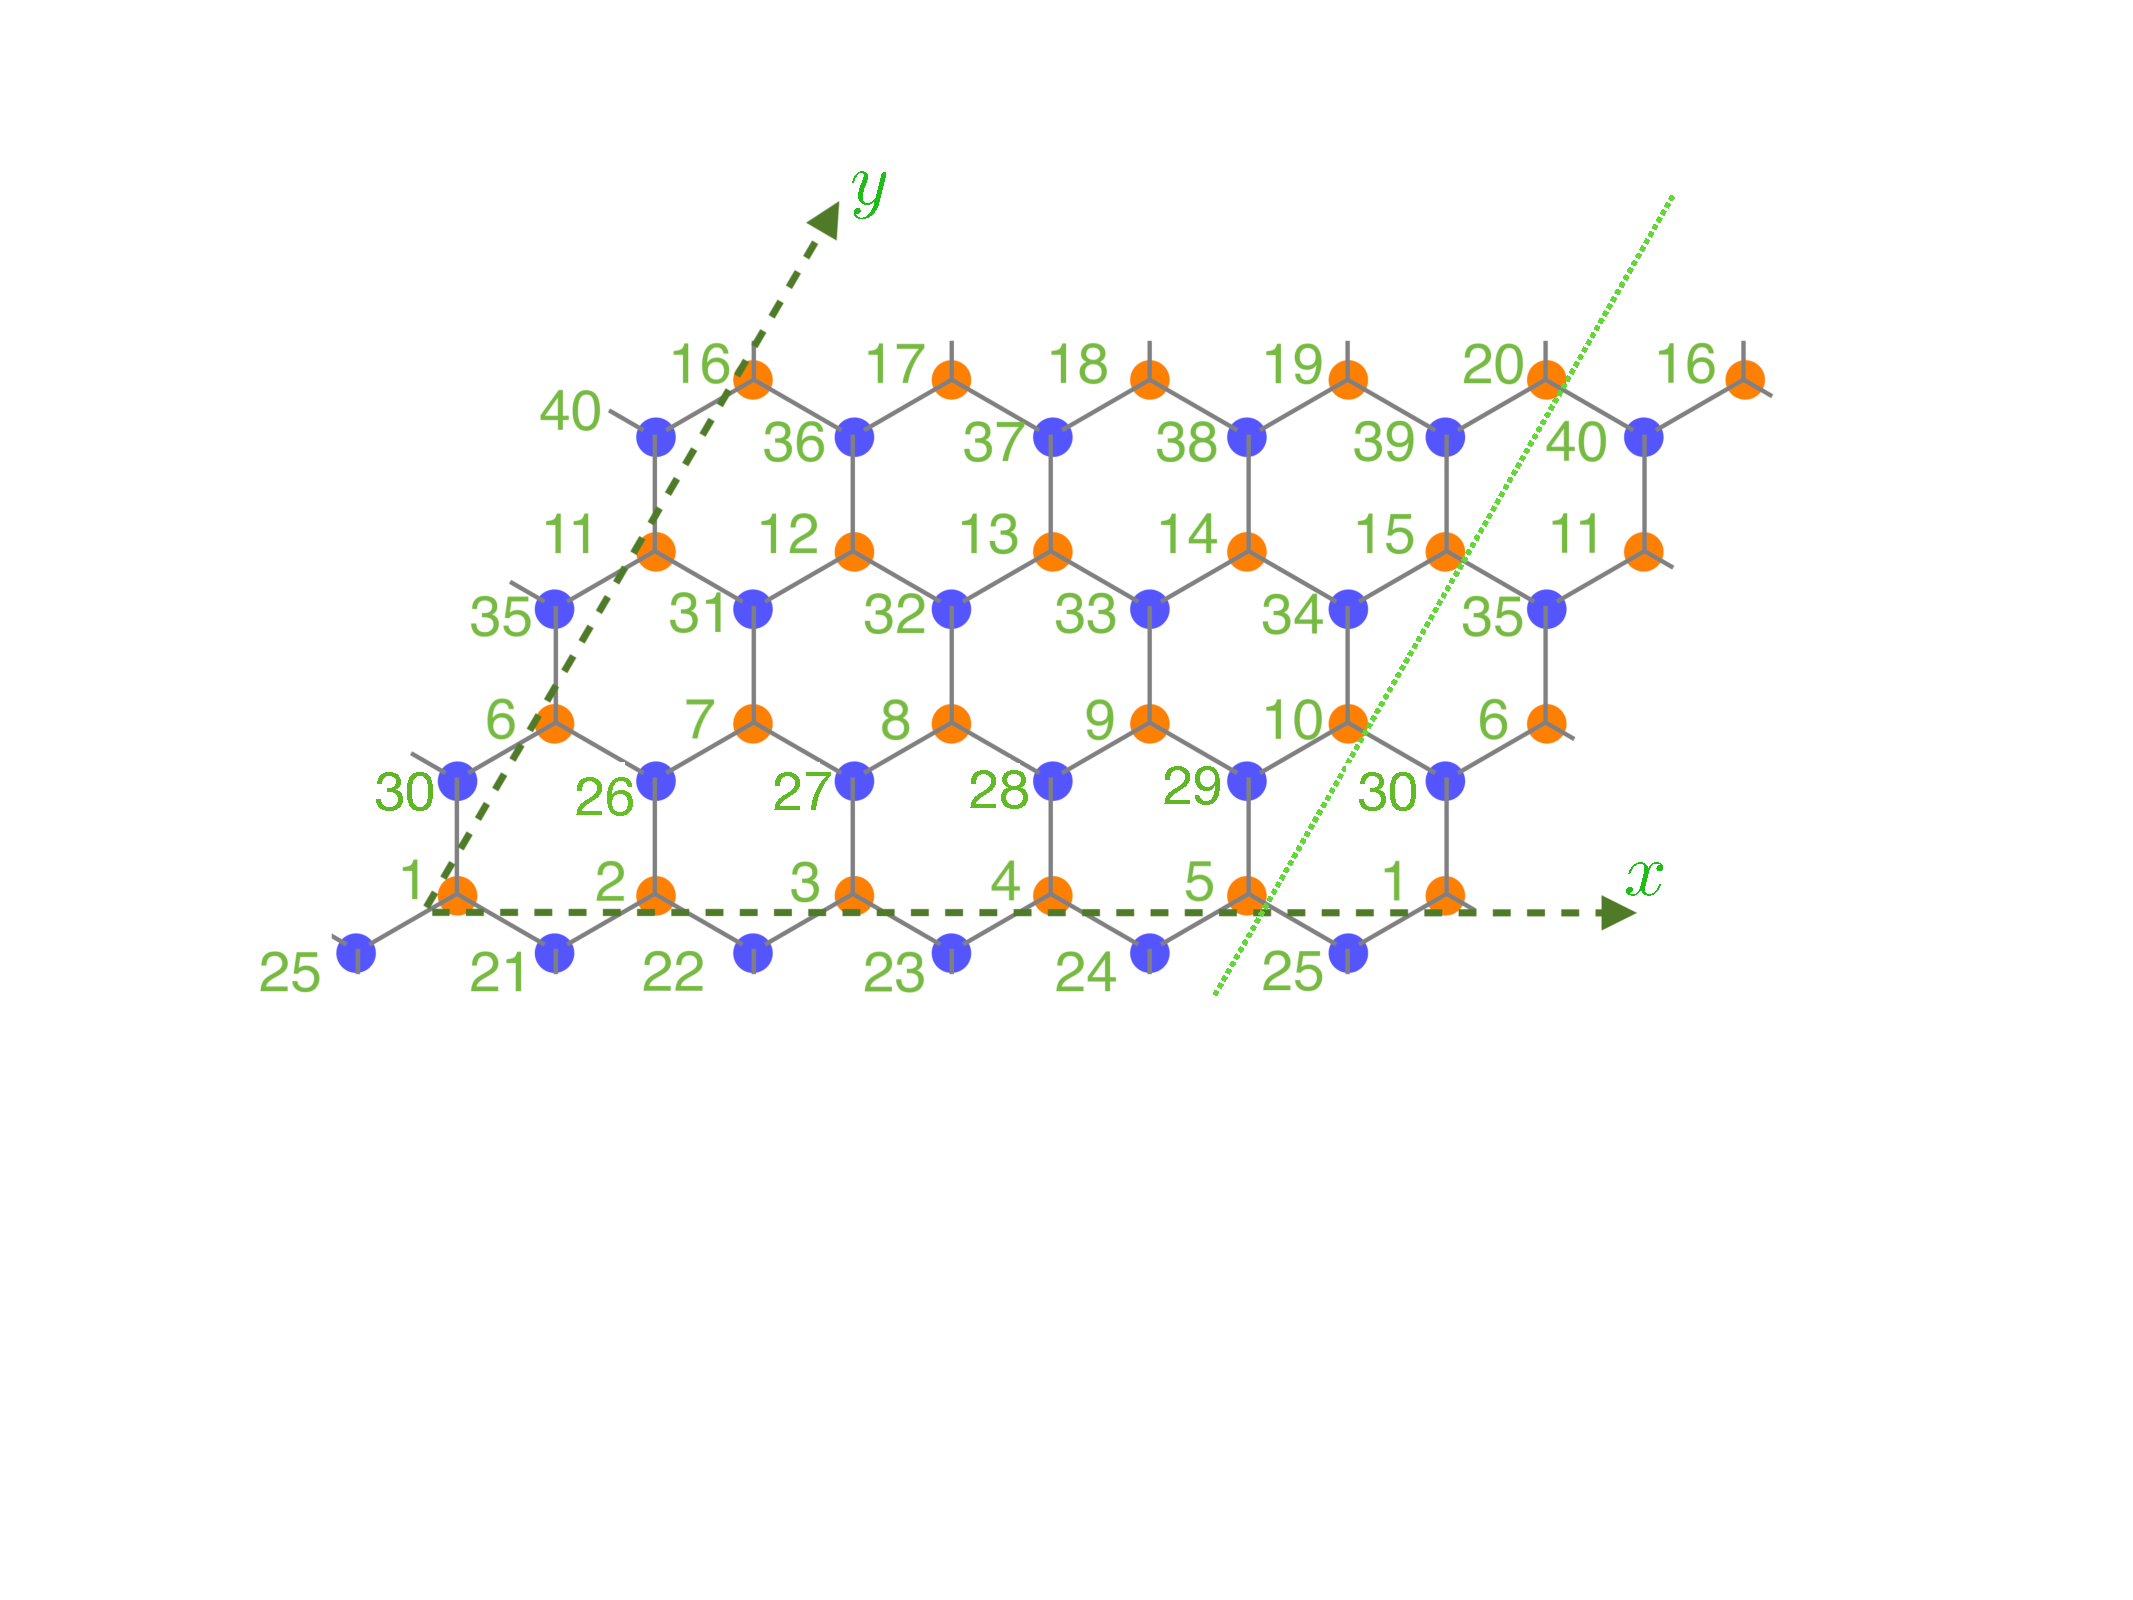
\includegraphics[trim={0 9cm 0 2.5cm},clip, width=0.8\linewidth]{Applications/nanoribbon.pdf}
	\caption[Boundary conditions on the nanoribbon.]{An illustration of the boundary conditions on the nanoribbon for $N_x = 5, \, N_y = 4$. Let the orange circles correspond to sublattice $A$, and the blue circles correspond to sublattice $B$.}
	\label{fig:nanoribbon}
\end{figure}

The geometry of the system appears through the hopping matrix $\bm K$ in our code.
The elements of the hopping matrix are simply defined by the indicator function: $K_{ij} = \mathbbm{1}_{\left\langle j_i \right\rangle} (i)$, where $\left\langle j_i \right\rangle$ is the set of neighbors $j$ of site $i$.
This numbering system makes it straightforward to find the neighbors of each site.
Let us begin by considering a site that is not on a zigzag edge.
There are four possible cases. For example, for 

\begin{equation*}
z_i = 0, y_i \neq N_y - 1, x_i \neq 0 ,
\end{equation*}
we have $\left\langle j_i \right\rangle = \{ j ( \bm r) \}$, with $\bm r$ in
\begin{equation*}
\bigg\{ \bm r_j \in \mathcal{L} \bigg| z_j = 1 \,\land\, \bigg[ \bigg( y_j = y_i  \,\land\, ( x_j = x_i \,\lor\, x_j = x_i - 1) \bigg) \,\lor\, \bigg( y_j = y_i + 1  \,\land\, x_j = x_i - 1  \bigg)  \bigg] \bigg\}
\end{equation*}

As opposed to the sites of a honeycomb lattice with \acp{PBC}, which have 3 neighbors, the sites of the zigzag edges have only 2 neighbors.
Again, there are four possible cases. For example, for 

\begin{equation*}
z_i = 0, y_i = N_y - 1, x_i \neq 0 ,
\end{equation*}
we have $\left\langle j_i \right\rangle = \{ j ( \bm r) \}$, with $\bm r$ in
\begin{equation*}
\bigg\{ \bm r_j \in \mathcal{L} \bigg| z_j = 1 \,\land\, y_j = y_i  \,\land\, ( x_j = x_i \,\lor\, x_j = x_i - 1) \bigg\}
\end{equation*}

We summarize these and the remaining cases in the following table.

\begin{table}[H]
	\hspace{-2.5cm}
	\caption{Nearest neighbors on the nanoribbon.}
	\begin{tabular}{|c|c|c|c|} \hline
	\multicolumn{4}{|c|}{\textbf{\acp{PBC}}}							\\ \hline
		Case 				& $z_j$	& $y_j$	& $x_j$ 	\\ \hline
		\multicolumn{1}{|c|}{\multirow{3}{*}{$z_i = 0, y_i \neq N_y - 1, x_i \neq 0$}}	 &	\multicolumn{1}{c|}{\multirow{3}{*}{1}} & \multicolumn{1}{c|}{\multirow{2}{*}{$y_i$}} & $x_i$   \\ \cline{4-4}
	   	\multicolumn{1}{|c|}{}	& \multicolumn{1}{c|}{\multirow{3}{*}{}} & \multicolumn{1}{c|}{\multirow{2}{*}{}}& \multicolumn{1}{c|}{\multirow{2}{*}{$x_i - 1$}} \\ \cline{3-3}
	   	\multicolumn{1}{|c|}{}	& \multicolumn{1}{c|}{} & $y_i +1$ & \multicolumn{1}{c|}{\multirow{2}{*}{}} \\ \hline
		\multicolumn{1}{|c|}{\multirow{3}{*}{$z_i = 0, y_i \neq N_y - 1, x_i = 0$}}	 &	\multicolumn{1}{c|}{\multirow{3}{*}{1}} & \multicolumn{1}{c|}{\multirow{2}{*}{$y_i$}} & 0   \\ \cline{4-4}
	   	\multicolumn{1}{|c|}{}	& \multicolumn{1}{c|}{\multirow{3}{*}{}} & \multicolumn{1}{c|}{\multirow{2}{*}{}}& \multicolumn{1}{c|}{\multirow{2}{*}{$N_x - 1$}} \\ \cline{3-3}
	   	\multicolumn{1}{|c|}{}	& \multicolumn{1}{c|}{} & $y_i +1$ & \multicolumn{1}{c|}{\multirow{2}{*}{}} \\ \hline
		\multicolumn{1}{|c|}{\multirow{3}{*}{$z_i = 1$, $y_i \neq 0$, $x_i \neq N_x - 1$}}	 &	\multicolumn{1}{c|}{\multirow{3}{*}{1}} & \multicolumn{1}{c|}{\multirow{2}{*}{$y_i$}} & $x_i$   \\ \cline{4-4}
	   	\multicolumn{1}{|c|}{}	& \multicolumn{1}{c|}{\multirow{3}{*}{}} & \multicolumn{1}{c|}{\multirow{2}{*}{}}& \multicolumn{1}{c|}{\multirow{2}{*}{$x_i + 1$}} \\ \cline{3-3}
	   	\multicolumn{1}{|c|}{}	& \multicolumn{1}{c|}{} & $y_i +1$ & \multicolumn{1}{c|}{\multirow{2}{*}{}} \\ \hline
		\multicolumn{1}{|c|}{\multirow{3}{*}{$z_i = 1$, $y_i \neq 0$, $x_i = N_x - 1$}}	 &	\multicolumn{1}{c|}{\multirow{3}{*}{1}} & \multicolumn{1}{c|}{\multirow{2}{*}{$y_i$}} & $N_x - 1$   \\ \cline{4-4}
	   	\multicolumn{1}{|c|}{}	& \multicolumn{1}{c|}{\multirow{3}{*}{}} & \multicolumn{1}{c|}{\multirow{2}{*}{}}& \multicolumn{1}{c|}{\multirow{2}{*}{0}} \\ \cline{3-3}
	   	\multicolumn{1}{|c|}{}	& \multicolumn{1}{c|}{} & $y_i -1$ & \multicolumn{1}{c|}{\multirow{2}{*}{}} \\ \hline
	\end{tabular}
	\hspace{-0.1cm}
	\begin{tabular}{|c|c|c|c|} \hline
	\multicolumn{4}{|c|}{\textbf{\acp{OBC}}}							\\ \hline
		Case 				& $z_j$	& $y_j$	& $x_j$ 	\\ \hline
	\multicolumn{1}{|c|}{\multirow{2}{*}{$z_i = 0, y_i = N_y - 1, x_i \neq 0$}}	 &	\multicolumn{1}{c|}{\multirow{2}{*}{1}} & \multicolumn{1}{c|}{\multirow{2}{*}{$y_i$}} & $x_i$   \\ \cline{4-4}
	   	\multicolumn{1}{|c|}{}	& \multicolumn{1}{c|}{\multirow{2}{*}{}}  & \multicolumn{1}{c|}{}& $x_i - 1$ \\ \hline
	   	\multicolumn{1}{|c|}{\multirow{2}{*}{$z_i = 0, y_i = N_y - 1, x_i = 0$}}	 &	\multicolumn{1}{c|}{\multirow{2}{*}{1}} & \multicolumn{1}{c|}{\multirow{2}{*}{$y_i$}} & 0   \\ \cline{4-4}
	   	\multicolumn{1}{|c|}{}	& \multicolumn{1}{c|}{\multirow{2}{*}{}}  & \multicolumn{1}{c|}{}& $N_x - 1$ \\ \hline
	   	\multicolumn{1}{|c|}{\multirow{2}{*}{$z_i = 1, y_i = 0, x_i \neq N_x - 1$}}	 &	\multicolumn{1}{c|}{\multirow{2}{*}{1}} & \multicolumn{1}{c|}{\multirow{2}{*}{$y_i$}} & $x_i$   \\ \cline{4-4}
	   	\multicolumn{1}{|c|}{}	& \multicolumn{1}{c|}{\multirow{2}{*}{}}  & \multicolumn{1}{c|}{}& $x_i + 1$  \\ \hline
	   	\multicolumn{1}{|c|}{\multirow{2}{*}{$z_i = 1, y_i = 0, x_i = N_x - 1$}}	 &	\multicolumn{1}{c|}{\multirow{2}{*}{1}} & \multicolumn{1}{c|}{\multirow{2}{*}{$y_i$}} & 0   \\ \cline{4-4}
	   	\multicolumn{1}{|c|}{}	& \multicolumn{1}{c|}{\multirow{2}{*}{}}  & \multicolumn{1}{c|}{}& $N_x - 1$ \\ \hline
	\end{tabular}
	\label{tab:dummytable}
\end{table}


